\section{Theory}

While the SM model demonstrates promising empirical results \cite{Gasthaus} we are unsatisfied with the linear space requirement for reasons stated earlier.  We propose a framework for limiting the memory required to represent models based on the hierarchical Pitman-Yor process.  Estimation in this framework can be viewed either as a valid inference scheme for a model based on a dependent set of hierarchical Pitman-Yor processes or as an approximate inference technique for a non-varying model.

\subsection{Dependent Pitman-Yor process} 

The $\ES_N(d,c)$ distribution discussed in Section~\ref{basicModel} has an important consistency property. In the Chinese restaurant metaphor the consistency property corresponds to the fact that if a customer is removed uniformly at random, the remaining customer configuration represents a partition of the integer $N-1$ following the $\ES_{N-1}(d,c)$ distribution. Another deletion operation known as size-biased deletion, in which a customer is chosen uniformly at random and all customers seated at the same table are removed from the restaurant, is known to satisfy such a consistency property for the one parameter Ewen's distribution \cite{kingman}.  This is known as the species deletion property \cite{kingman}, but does not hold in the two parameter case \cite{pitman}

The consistency property allows the restaurant metaphor to be generalized to aid in producing samples at discrete points $t = 1 \dots T$ from a dependent random distribution $\G^t_1$ such that $\G^t_1 \sim \PY(d_1, c_1, \G_0)$ for all $t$.   The fact that $\G^t_1$ has the same distribution over time is known as stationarity in the time-series literature \cite{davis and brockwel?}.  The process works by marginalizing out $\G^t_1$ at all time points and drawing dependent samples.

The process, an extension of the analogous process for Dirichlet processes \cite{caron}, starts with an empty restaurant and generates $x^1_1 \dots x^1_{n(1)}$ through the typical Chinese restaurant process.  Between time points customers are deleted uniformly at random from the state of the restaurant.  After deletion, the sample for the next time point is drawn using the Chinese restaurant process starting with the state of the restaurant after the deletion step.  Because of the consistence property, if $j$ customers are deleted after time step 1 the random partition represented by the starting state of the restaurant at time step 2 has a $\ES_{n(1) - j}(d,c)$ distribution.  The seating process at time step 2 maintains the correct $\ES$ distribution, creating samples drawn from $\G^2_1 \sim \PY(d,c,\G_0)$.  Not that the number of customers removed from the restaurant between time steps is independent of the consistence result and can thus be either stochastic or deterministic.

Dependence between $\G_t^1$ arises from the generalized urn scheme through the undeleted customers.  Exact characterization of the dependence induced by the process is non-trivial, though it is clear that fewer customers removed between times steps induces higher dependence.  In the extreme cases, removing all the customers between time steps gives draws from independent $\G_t^1$, while removing no customers induces a $\G_1$ that is not varying with time. Some exploration is done in \cite{caron} of the dependence structure for the analogous Dirichlet process restaurant scheme.

%TODO give graphical model
\subsection{Time-varying Pitman-Yor Process in a hierarchical setting}

The time-varying framework can be extended to a hierarchical setting at the lowest level of hierarchy in a natural way.  Considering the simple hierarchical setting $\G_2 \sim \PY(d_2, c_1, \G_1)$ and $\G_1 \sim \PY(d_1, c_1, \G_0)$, the model may be generalized to $\G^t_2 \sim  \PY(d_2, c_1, \G_1)$ for all $t  = 1 \dots T$.  One specification of this model is to combine the Chinese restaurant franchise process with the generalized restaurant process.  In this representation customers are removed from the restaurant correspond to $\G_2$ between time steps.  The restaurant corresponding the $\G_1$ is unchanged between time steps. Samples are drawn according the Chinese restaurant franchise already outlined at each time step.

\begin{figure}[h!tbp] 
	\begin{center}
		\scalebox{.25}{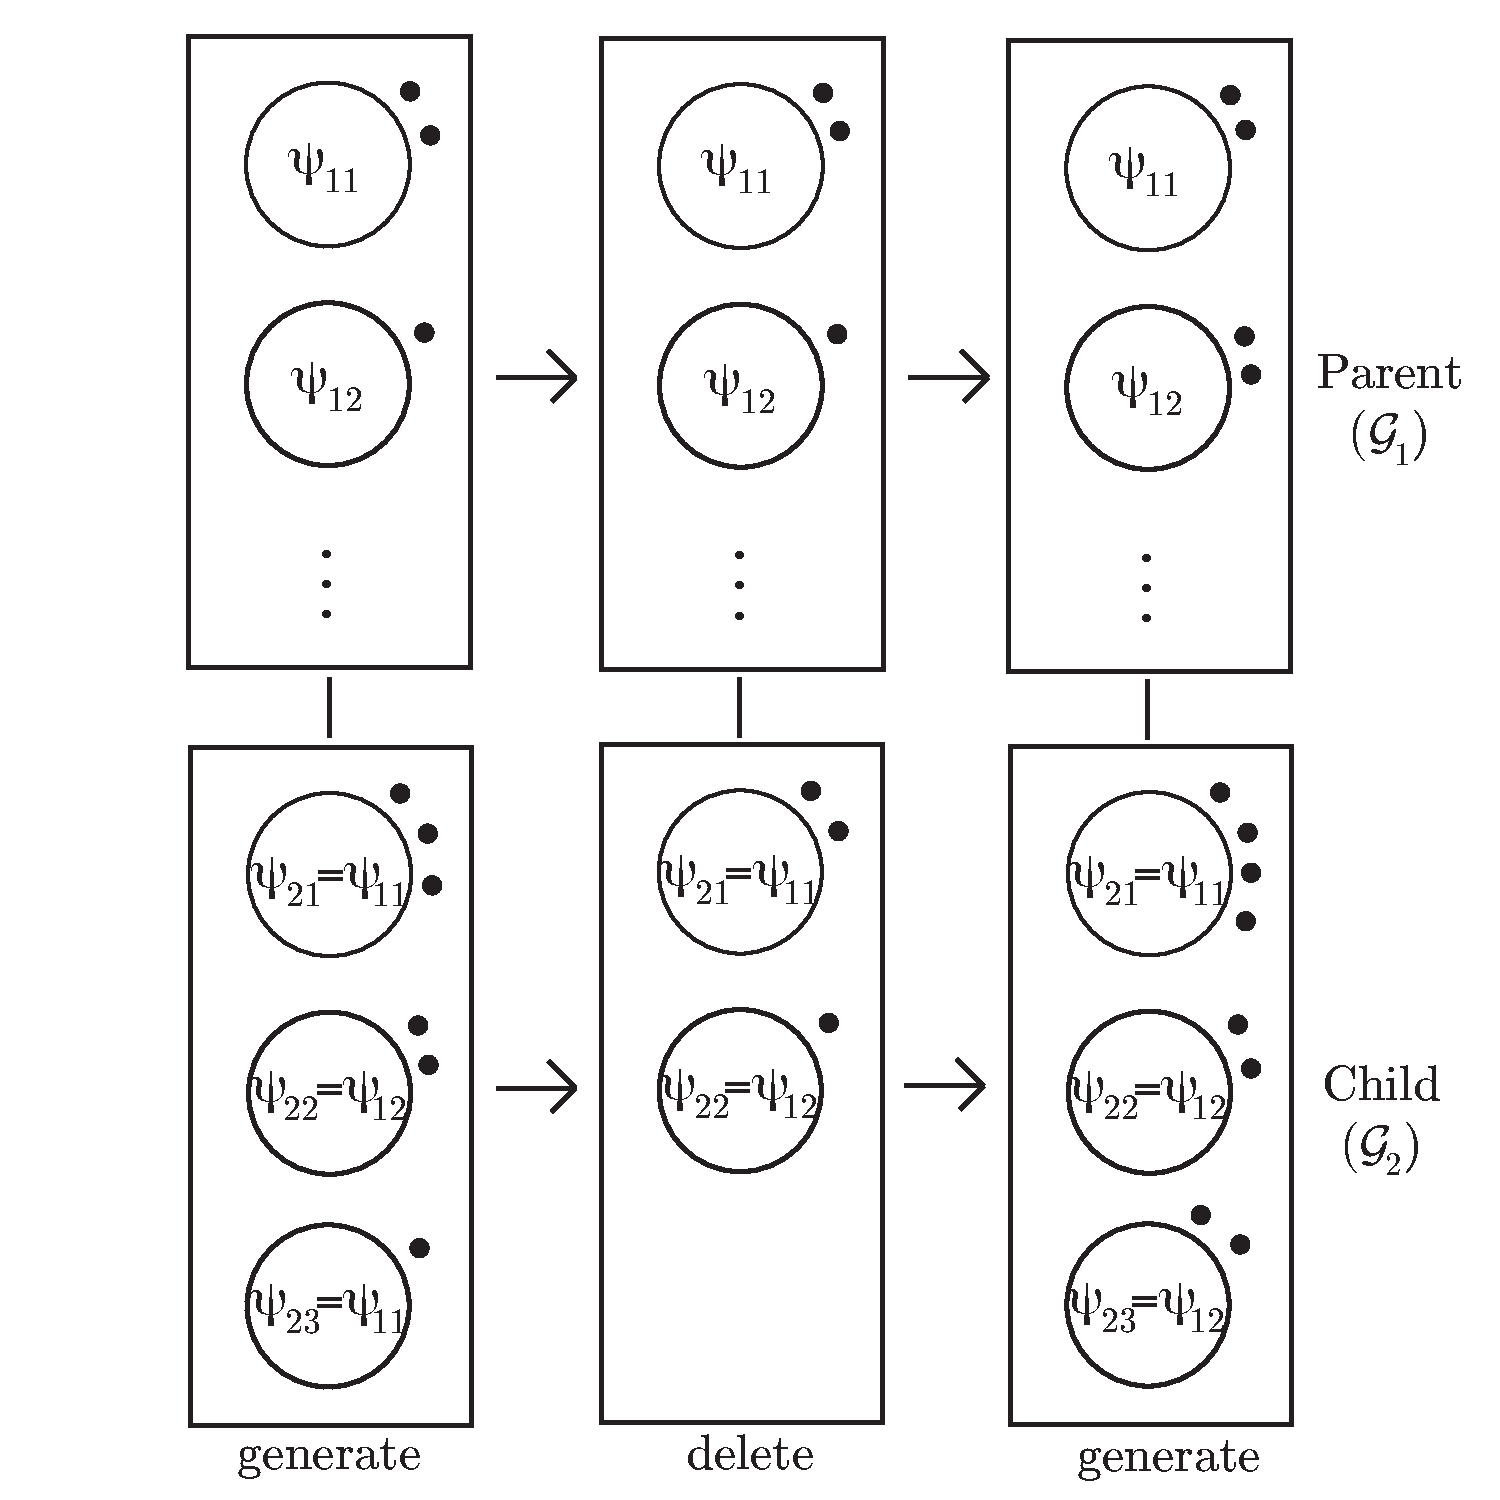
\includegraphics{figure2.pdf}} % [clip=true, viewport= 1in 1in 9in 9in]
		\caption{An example of the possible evolution of the restaurant states in hierarchical setting}
	\end{center} 
	\label{figVHPY}
\end{figure} 

Only simple extensions allow for time-varying distributions higher on the hierarchy are clear.  For a model specification such as $\G_2^t \sim \PY(d_2, c_2, \G_1^t)$ and $\G_1^t  \sim \PY(d_1,d_2,\G_0)$ for all $t$, if we assume independence of the $\{ \G_2^t \}$ then we can employ the generalized restaurant scheme to create a time-varying dependent sequence of restaurant representations at the  $\G_1^t$ level and at each time start with an empty restaurant for the representation used to marginalize out $\G_2^t$.  However, it is not clear how to create dependence at the $\G_2^t$ level through the generalized restaurant process.  Such a restaurant scheme would require a process to update the restaurant state in the $\G_2^t$ level restaurant to reflect changes made to the state of the $\G_1^t$ level restaurant while maintaining a level of dependence.  While it is likely that such a process exists, it is neither intuitive nor necessary for this discussion.

\subsection{Time-varying model applied to SM}

The time-varying model will not only allow for a sequence of time-varying distributions, but can also serve to limit the complexity of the model representation. This framework provides a basis for algorithmic control of the complexity of hierarchical Pitman-Yor models like the SM.  As noted earlier, the number of instantiated restaurants in the SM is the fundamental limiting factor regarding memory usage, thus we will consider a single instantiated restaurant as a unit of memory when discussing the model. For the deletion scheme to limit the amount of memory used by the SM model, we must be able to limit the number of instantiated restaurants.

\begin{figure*}[t] 
	\begin{center}
		\scalebox{.4}{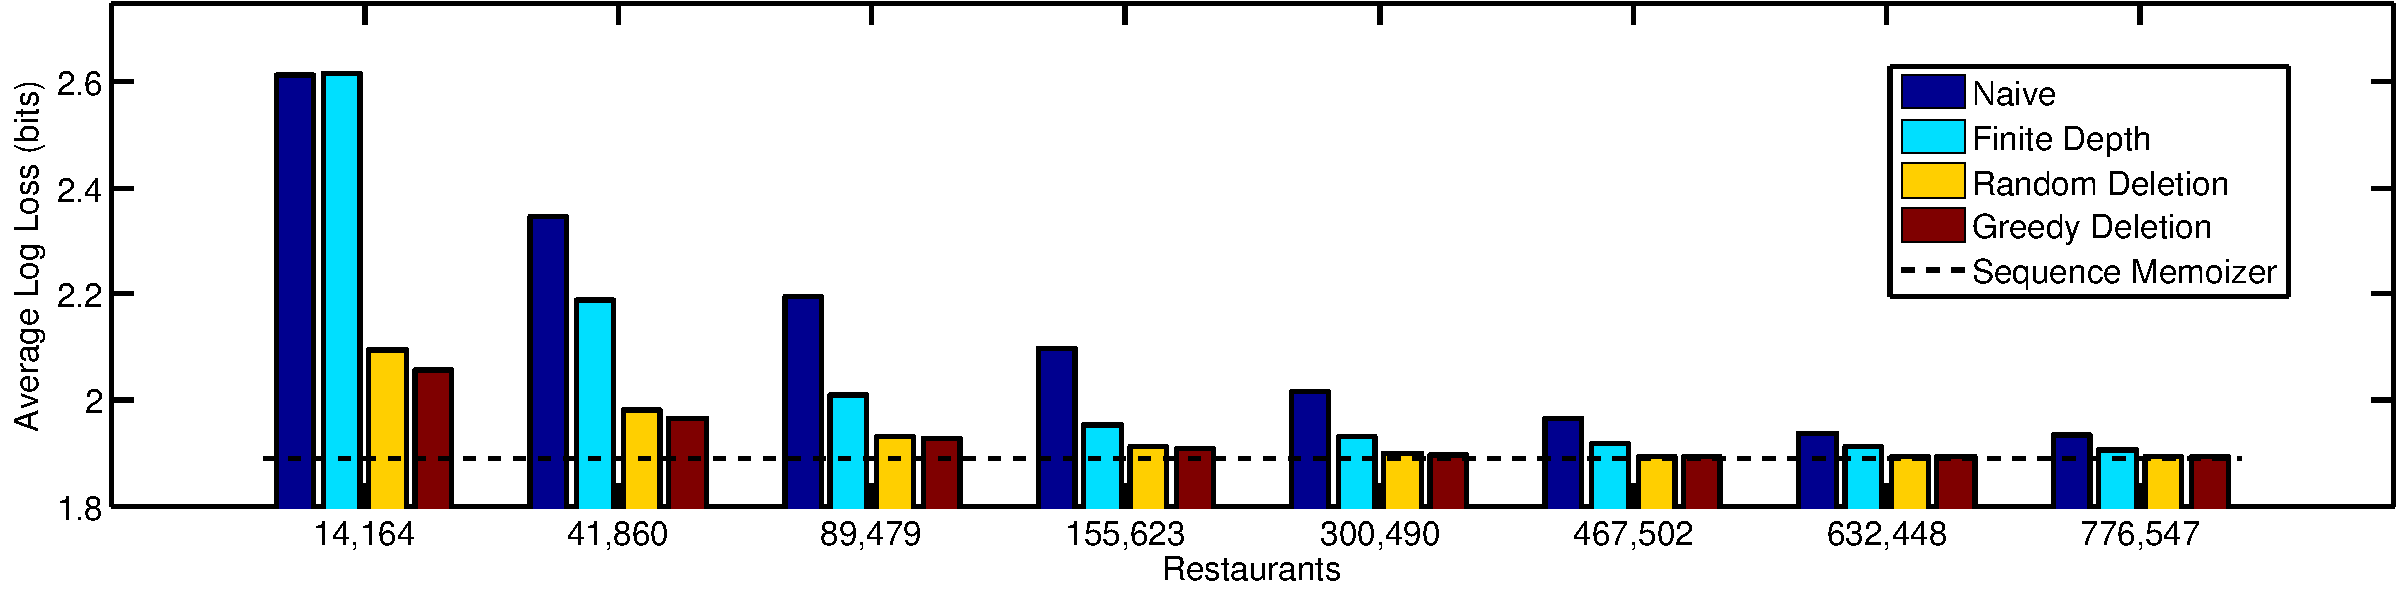
\includegraphics{results_calgary_corpus.pdf}} % [clip=true, viewport= 1in 1in 9in 9in]
		\caption{An example of the possible evolution of the restaurant states in hierarchical setting}
	\end{center} 
	\label{figResultsCC}
\end{figure*} 

The theory presented above indicates that between time steps we can only delete customers in restaurants at the lowest level.  In the tree which represents the state of the SM, this corresponds to the leaf restaurants.  To achieve memory savings we will need to delete all of the customers at a given restaurant.  Restaurants without people need not be represented in the model state.  This deletion operation gives rise to implicit model assumptions. If, at time step $t$, we delete all the customers in a given leaf restaurant we implicitly assume the distribution over types given the particular context to be independent of the distribution at previous time steps.

It is often the case in the SM model that the parent restaurant for a leaf restaurant is not instantiated, thus to actually attain memory savings by deleting a leaf restaurant we must effectively delete all the restaurants in this particular path up until the nearest instantiated restaurant.  The implicit model assumption is that all of the distributions after time $t$ corresponding to those many deleted restaurants are conditionally independent of their previous states.

This is the basic framework for both bounded memory algorithms we present and is the main contribution of this paper.  The assumption that, for many contexts, the distribution changes over time seems appropriate for very long sequences. The assumption of independence required for us to justify our particular deletion process is primarily of practical motivation though we expect information lost to be minimal. 

Finally, we point out that the theory behind these deletion operations holds for general hierarchical Pitman-Yor processes and thus also for finite depth n-gram style models.  In Section~\ref{results} we show some results concerning this type of model as well.
